\algorithm{The Degrading Obfuscation Algorithm}%
          {D. Mandel, A. Segurson}


\section{Introduction}
The Degrading algorithm for obfuscation is designed to slow down java
applications. It consists of two main parts, the promotion obfuscator,
and the thread contention obfuscator. There is a motivation behind the
desire to make java applications run slower: Software company X wants to
release a new program. But, company X wants the users to be able to
try the new software before they buy it, as a motivation to own it.
If the customer already has a working version of the software, why
would they still buy it? Because company X only released a slightly
crippled version of the software and the customer will enjoy  
the optimal speed of the full version. Thus, company X will degrade
their product and release it as a free demo, and sell the fastest
working version.

What makes java programs run slower? Memory managment, and thread 
contention are two things in java code that we focus on that 
can slow things down.
Our goal is to increse the amount of these two things in the java
application with some control.

The following is the discussion of the two algorithms used in the 
Degrading Obfuscation, followed by some analysis of programs in which 
the degradation was applied.

\section{Promotion Obfuscation}
The main goal of the promotion obfuscator is to increase the amount
of memory management in the java application. Almost everything in
java is already an object, so the target was clear: primitive local
variables. Primitive local variables are used quite frequently in
programming, which in java includes the types: ``\texttt{
boolean}, \texttt{byte}, \texttt{char}, \texttt{int},
\texttt{double}, \texttt{float}, \texttt{long}, and \texttt{short}."
Luckily, java already has provided us with objects that can hold these
values. 

The details on how to promotote the primitive local variables to an
object local variables 
vary slightly from primitive to primitive. The basic idea follows
these steps:
\begin{itemize}
  \item cast all primitive variable parameters passed into the method to
    local objects 
  \item when a primitive variable is loaded, replace the load with
    a call to the local object's value function
  \item when a primitive variable is stored, replace the store with
    a constructor for a new object and store the new object
\end{itemize}

\subsection{Special \texttt{int}'s}
The primitive \texttt{int} is probably the most common used
primitive for a local variable. Also, on the java byte code
level the primitives \texttt{boolean}, \texttt{byte},
\texttt{char}, and \texttt{short} are treated exactly the same as
\texttt{int} variables. See the figure for an example. So, there
is no support for \texttt{boolean}, \texttt{byte}, \texttt{char},
and \texttt{short}'s on the byte code level, they are all 
\texttt{int}'s. 

\begin{figure}[ht]
\begin{listing}{1}
   public static char myMethod(short b, int c, boolean bb) {
      if (bb) {
         int x = b + c;
         return 'a';
      }
      return 'b';
   }
\end{listing}{1}
\begin{listing}{1}
.method public static myMethod(SIZ)C
.limit stack 2
.limit locals 4

Label1:
.line 7
        iload_2
        ifeq Label0
.line 8
        iload_0
        iload_1
        iadd
        istore_3
.line 9
        bipush 97
        ireturn
Label0:
.line 11
        bipush 98
Label2:
        ireturn

.end method
\end{listing}{1}
\caption{The listing of the java, and the java byte code for the method,
  \texttt{myMethod}. \texttt{myMethod}'s signature in the byte code 
  accepts a \texttt{short}, \texttt{int} and a \texttt{boolean}
  as paramaters, but when the method uses these
  paramaters it always uses an \texttt{iload}. Also, when
  the method returns the \texttt{char} it uses an \texttt{ireturn}.}
\end{figure}

As a result of java's treatment of the small primitives (
\texttt{boolean},
\texttt{byte},
\texttt{char}, and
\texttt{short}),
the small primitives can all be stored in the object, \texttt{Integer}.
There are objects for all of the small primitives, but detailed 
analysis of the program would be required to use the same 
object as small primitive, and there would be no beneficial results.
For example, one could do data analysis on the local variable $2$, and
if it is an integer which is always $0$ or $1$ then it could be stored
in a \texttt{Boolean} object, but saving it in the  \texttt{Boolean} object
offers no advantage over saving it in a \texttt{Integer} object. For
the rest of the section \texttt{int}'s will include all small primitives.

\subsection{Promoting Primitives}
There are only four main types of primitives: \texttt{int}, 
\texttt{float}, \texttt{long} and \texttt{double}. To implement the
promotion obfuscator four method obfuscator algorithms were added
to Sandmark:
\begin{itemize}
  \item DPromote - \texttt{double} promote
  \item FPromote - \texttt{float} promote
  \item IPromote - \texttt{int} promote
  \item LPromote - \texttt{long} promote
\end{itemize}
All four method obfuscator algorithms begin by loading all of the 
primitive parameters into an object. Figure \ref{params} is the new byte
code created for each primitive paramter type at the beginning of the method.

\begin{figure}[ht]
\begin{tabular}{| l | l |}
\hline
\textbf{Long} & \textbf{Float} \\
\hline
\texttt{new java/lang/Long} & \texttt{new java/lang/Float} \\
\texttt{dup} & \texttt{dup} \\
\texttt{lload 4} & \texttt{fload\_2} \\
\texttt{invokespecial java/lang/Long/<init>(J)V} & \texttt{invokespecial java/lang/Float/<init>(F)V} \\
\texttt{astore 4} & \texttt{astore\_ 2} \\
\hline
\textbf{Int} & \textbf{Double} \\
\hline
\texttt{new java/lang/Integer} & \texttt{new java/lang/Double} \\
\texttt{dup} & \texttt{dup} \\
\texttt{iload\_3} & \texttt{dload\_0} \\
\texttt{invokespecial java/lang/Integer/<init>(I)V} & \texttt{invokespecial java/lang/Double/<init>(D)V} \\
\texttt{astore\_3} & \texttt{astore\_0} \\
\hline
\end{tabular}
\caption{The code inserted at the beginning of the method for each of
the four primitive types. In this example the signature of the static
method was  \texttt{myMethod(DFIJ)V}.}
\label{params}
\end{figure}

Now, there are only local variables that are objects. But, we still have
to change the rest of the method to correct the stores and loads to
reference the objects, instead of the primitives.  
Figures \ref{subs} - \ref{endsubs} itemize all the substitutions
that need to be made.
\begin{center}
\begin{figure}[h]
\begin{tabular}{| l | l |}
   \hline
   Old Byte Code & Replacement Byte Code \\
   \hline
   \texttt{istore \textless index\textgreater} & \texttt{new Ljava/lang/Integer;} \\
      & \texttt{dup\_x1} \\
      & \texttt{dup\_x1} \\
      & \texttt{pop} \\
      & \texttt{invokespecial java/lang/Integer/\textless init\textgreater(I)V} \\
      & \texttt{astore \textless index\textgreater} \\
   \hline
   \texttt{iload \textless index\textgreater} & \texttt{aload \textless index\textgreater} \\
      & \texttt{invokevirtual java/lang/Integer/intValue(V)I} \\
   \hline
   \texttt{iinc \textless index\textgreater \textless num \textgreater}
      & \texttt{new Ljava/lang/Integer;}  \\
      & \texttt{dup}  \\
      & \texttt{ldc \textless num\textgreater}   \\
      & \texttt{aload \textless index\textgreater}   \\
      & \texttt{invokevirtual java/lang/Integer/intValue(V)I}  \\
      & \texttt{iadd}  \\
      & \texttt{invokespecial java/lang/Integer/\textless init\textgreater (I)V } \\      & \texttt{astore \textless index\textgreater}  \\
   \hline
\end{tabular}
\caption{Substitution for integers.}
\label{subs}
\end{figure}
\begin{figure}[htb]
\begin{tabular}{| l | l |}
   \hline
   Old Byte Code & Replacement Byte Code \\
   \hline
   \texttt{lstore \textless index\textgreater} & \texttt{new Ljava/lang/Long;} \\
      & \texttt{dup\_x2} \\
      & \texttt{dup\_x2} \\
      & \texttt{pop} \\
      & \texttt{invokespecial java/lang/Long/\textless init\textgreater(J)V} \\
      & \texttt{astore \textless index\textgreater} \\
   \hline
   \texttt{lload \textless index\textgreater} & \texttt{aload \textless index\textgreater} \\
      & \texttt{invokevirtual java/lang/Long/longValue(V)J} \\
   \hline
\end{tabular}

\begin{tabular}{| l | l |}
   \hline
   Old Byte Code & Replacement Byte Code \\
   \hline
   \texttt{fstore \textless index\textgreater} & \texttt{new Ljava/lang/Float;} \\
      & \texttt{dup\_x1} \\
      & \texttt{dup\_x1} \\
      & \texttt{pop} \\
      & \texttt{invokespecial java/lang/Float/\textless init\textgreater(F)V} \\
      & \texttt{astore \textless index\textgreater} \\
   \hline
   \texttt{fload \textless index\textgreater} & \texttt{aload \textless index\textgreater} \\
      & \texttt{invokevirtual java/lang/Float/floatValue(V)F} \\
   \hline
\end{tabular}

\begin{tabular}{| l | l |}
   \hline
   Old Byte Code & Replacement Byte Code \\
   \hline
   \texttt{dstore \textless index\textgreater} & \texttt{new Ljava/lang/Double;} \\
      & \texttt{dup\_x2} \\
      & \texttt{dup\_x2} \\
      & \texttt{pop} \\
      & \texttt{invokespecial java/lang/Double/\textless init\textgreater(D)V} \\
      & \texttt{astore \textless index\textgreater} \\
   \hline
   \texttt{dload \textless index\textgreater} & \texttt{aload \textless index\textgreater} \\
      & \texttt{invokevirtual java/lang/Double/doubleValue(V)D} \\
   \hline
\end{tabular}
\caption{Substitution for longs, floats and doubles.}
\label{endsubs}
\end{figure}
\end{center}


\newpage
\subsection{Controling Promotion}
The number of local variables that are promoted can be controled to
a limited extent. The following parameter can be set in the Degrade
configuration:
\begin{itemize} 
  \item \texttt{OBF\_DE\_PERCENT} - The approximate percent of the
    primitive local variables that you want to promote.
\end{itemize} 
The algormithm will then apply the promotion obfuscation to methods
in the jar file until it has reached or exceeded the desired percent.
It uses the greedy algorithm to achieve this.

\newpage
\section{Thread Contention Obfuscation}

This algorithm attempts to automagically slow down some method in a program
by inserting threads that perform busy-waiting while the original code in the
method runs.  While the idea of slowing down a program may seem odd, commercial
software developers may find this idea interesting in order to give away a
slower version of their product while charging for the complete version.  This
algorithm may also be used as a benchmarking scheme for java's multithreaded
features.  In
addition, the obfuscation value of this algorithm (when it is completely
implemented with sufficient stealthiness) should not be underestimated.
Multithreaded code has been known to confuse even advanced programmers, and
obfuscated multithreaded code should further help in this quest for confusion.


\begin{figure}
\begin{center}
\resizebox{4in}{!}{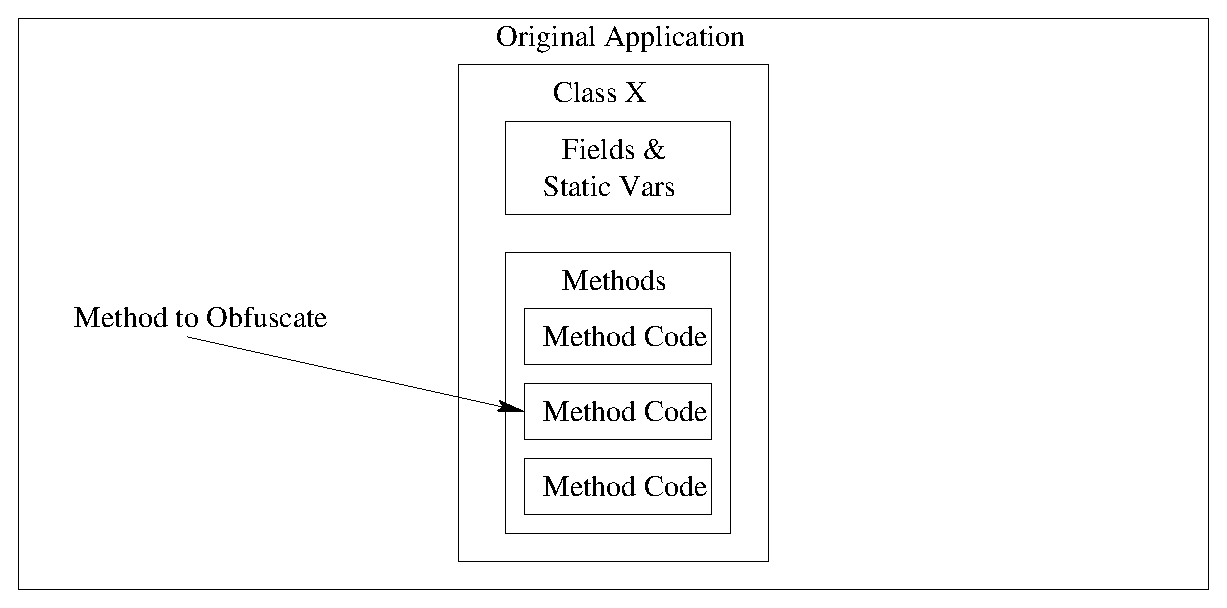
\includegraphics{FIGS/TCoriginal.eps}}
\end{center}
\caption{The original application to obfuscate.  A method is selected for
obfscation}
\end{figure}

\begin{figure}
\begin{center}
\resizebox{4in}{!}{\includegraphics{FIGS/TCobf.eps}}
\end{center}
\caption{The application after obfuscation.  The original method's code has 
been moved to a thread which the original method now starts.  An Integer-like
class has been added for locking purposes.}
\end{figure}  


\subsection{Apply}
For the algorithm to work, the user must have configured the following
parameters beforehand:
\begin{itemize}
  \item \texttt{OBF\_TC\_ClassName} - The name of the class where the method
        resides
  \item \texttt{OBF\_TC\_MethodName} - The name of the method to obfuscate
  \item \texttt{OBF\_TC\_NumThreads} - The number of threads to insert into that
        method
\end{itemize}

\noindent
If a method with the given class and name isn't found, then the obfuscation
does nothing.  Once these values have been set, the user may run the algorithm.  A summary of the steps taken during the obfuscation are as follows:

\begin{itemize}
  \item A new \texttt{java.lang.Integer}-like class is added to the jar file
  \item A static initializer is either modified (if it already exists) or
        created (if it doesn't already exist) and a static lock variable is
        added to the original class
  \item A new inner-thread class that contains the original method code is
        added to the original class
  \item Some number of other inner-thread classes are added to the original
        class
  \item The original method is modified so it starts the new inner thread
        class and waits for that thread to complete
\end{itemize}

\subsubsection{New java.lang.Integer Class}
In order to support various locking methods, the first step in the obfuscation
is to add a class similar to \texttt{java.lang.Integer}.  The main difference
between the new class and java's version is that the new class can change the
value stored in the Integer object.  This difference is significant because it
allows a different way of coordinating threads.  Java's built-in
synchronization mechanism relies on monitors which function through object
locks.  For our purposes, we want to use this in addition to value-based
synchronization mechanisms.  The standard \texttt{java.lang.Integer} class
cannot support value-based locking due to the value being immutable once the object has been
created.  If one wishes to change the value of an Integer, one must create a
new Integer, which throws away the reference to the old Integer, which renders
the java's built-in object locking mechanism useless.

\subsubsection{Static Initializer and Lock Variable Modified or Added}
For locking to take place, there needs to be some sort of locking variable.
While typical locking in java uses the \texttt{synchronized} keyword in method
headers, this synchronizes on the \texttt{this} object associated with that
method, which defeats our purpose of having more than one thread attempting
to run while our original method is running.  To get around this, we introduce
a new static class variable of our Integer-like class that the methods can
synchronize on.  A static initializer is added to the class in order to
construct our new Integer variable.

\subsubsection{New Inner-Thread Class}
A new inner-thread class is created in order to run the old method code.  The
new class contains one method, \texttt{run()}, which is required in order to
implement the \texttt{java.lang.Runnable} interface.  The method body of the
\texttt{run()} method contains the instructions that were formerly in the
original method.  However, there are two slight details that make this process
difficult, and both of them stem from the signature of the \texttt{run()}
method required by \texttt{java.lang.Runnable}.  Since the signature of this
method is set, it is impossible to pass parameters or return a value in the
conventional manner.  The workaround for this is to add static class variables
to the original class so that both the original class and the new class can
access the values.  It should be noted that all generated code (with the
exception of the first thread class which always has the name
\texttt{<className>}\$Inner) has random identifier strings associated with
them.  As well, all generated code is declared static so as to be accessible
from both a static and dynamic context.  For parameter passing, if the code
to be edited originally looked like this:

\begin{listing}{1}
public class ParamPassingExample {
   public static void main(String[] args) {
      for (int i = 0; i < args.length; i++) {
         System.out.println(``Arg `` + i + `` = `` + args[i]);
      }
   }
}
\end{listing}

\noindent
Then we would add the new class and a static variable so the resulting code
and modified \texttt{main(String[])} method would look like this:

\begin{listing}{1}
public class ParamPassingExample {
   // New static variable added to mimic parameter-passing
   private static String[] d3345;

   public static void main(String[] args) {
      Thread newThread;
      ParamPassingExample$Inner inner;

      // Assign the parameters to the new static class variable
      d3345 = args;

      inner = new ParamPassingExample$Inner();
      newThread = new Thread(inner);
      newThread.start();     
   }

   private static class ParamPassingExample$Inner implements java.lang.Runnable {
      public void run() {
         // Assign the static class variable to a local for manipulation like
         // how a parameter would normally be manipulated
         String[] local = d3345;

         for (int i = 0; i < local.length; i++) {
            System.out.println(``Arg `` + i + `` = `` + args[i]);
         }
      }
   }
\end{listing}

\noindent
Return types are treated in a similar manner, in that a new static variable
is added to the class.  However, for return types to work correctly, the
modified original method must spin on the lock until the thread has completed.
To illustrate this, consider the following example:

\begin{listing}{1}
public class ReturnTypeExample {

   public static void main(String[] args) {
      System.out.println(``Square root of 25 is: `` + squareRoot(25));
   }

   public static double squareRoot(int value) {
      return Math.sqrt((double) value);
   }
}
\end{listing}

\noindent
After adding the lock variable and modifying the \texttt{squareRoot(int)}
method to construct the thread and spin until the thread has completed, we
have the following code:

\begin{listing}{1}
public class ReturnTypeExample {
   // New static variable for param-passing
   private static int d546;
   // New static variable for return-type
   private static double g6789;
   // New static lock variable
   private static ReturnTypeExample$n7632 k3452;

   // static initializer added to construct new lock variable
   static {
      k3452 = new ReturnTypeExample$n7632(0);
   }

   public static void main(String[] args) {
      System.out.println(``Square root of 25 is: `` + squareRoot(25));
   }

   public static double squareRoot(int value) {
      ReturnTypeExample$Inner inner;
      Thread thread;

      // Store the parameter in a static class variable
      d546 = value;
      // Then start the thread
      inner = new ReturnTypeExample$Inner();
      thread = new Thread(inner);
      thread.start();
      // Spin on the lock until the thread completes its work
      while (k3452.j213() != 1) {
      }
      // Then return the newly added static variable
      return g6789;
   }

   private class ReturnTypeExample$Inner implements java.lang.Runnable {
      public void run() {
         // Re-assign the value of the lock variable to 0 to delay execution
         // of other threads
         k3452.n4795(0);
         // Assign the parameters to a local variable
         int local = d546;
         // Then assign the original return value to our static class member
         g6789 = Math.sqrt(d546);
         // Then assign the lock value to 1 so other threads can complete
         k3452.n4795(1);
      }
   }

   // Integer-like class
   private class ReturnTypeExample$n7632 {
      private int myValue;

      public ReturnTypeExample$n7632(int value) {
         super();
         myValue = value;
      }

      // Getter method
      public int j213() {
         return myValue;
      }

      // Setter method
      public void n4795(int value) {
         myValue = value;
      }
   }
}
\end{listing}

\subsubsection{Other New Thread Classes}
Any other new thread classes created during the process will have a
\texttt{run()} method with an empty spin loop waiting until the original thread
has completed.  In future revisions of the algorithm, these additional threads
may have domain-specific code inside of the spin loops, but for now they are
relatively unstealthy.  As an example, here is a possible inner-thread class:

\begin{listing}{1}
private class SomeClass$s78 implements java.lang.Runnable {
   public void run() {
      // Just spin on some lock variable
      while (b321.m987() != 1) {
      }
   }
}
\end{listing}

\noindent
Of course, the original method would also be modified to start this thread
as well.

\section{Sample Results}
These experiments were performed on an Intel Pentium III 1.2 ghz machine
running Red Hat Linux 7.2.  The application that was obfuscated was the famous
Sieve of Eratosthenes, an algorithm used to compute all prime numbers up to
some {\bfseries n}.  In the test case, the {\bfseries n} used was 99999999.
\begin{center}
\begin{table}[h]
\begin{center}
\begin{tabular}{| l |l| l |}
\hline
\emph{Number of threads used} & \emph{Percent Promotion} &\emph{Seconds Needed} \\
\hline
1 (original) & 0.0 & 12 seconds \\
\hline
1 & 1.0 & 52 seconds \\
\hline
2 & 0.0 & 25 seconds \\
\hline
2 & 1.0 & 73 seconds \\
\hline
3 & 0.0 & 38 seconds \\
\hline
3 & 1.0 & 122 seconds \\
\hline
4 & 0.0 & 64 seconds \\
\hline
4 & 1.0 & 411 seconds \\
\hline
\end{tabular}
\caption{Sample results obtained using Degradation on the Sieve of Eratosthenes}
\end{center}
\end{table}
\end{center}


